\documentclass{beamer}

\usepackage{ucs}
\usepackage[utf8x]{inputenc}
\usepackage[T1]{fontenc}
\usepackage[english]{babel}

\usepackage{multirow}%	multirow
\usepackage[retainorgcmds]{IEEEtrantools}%	IEEEeqnarray
\usepackage{mathabx}%	convolution symbol
\usepackage{relsize}%	relative font sizes
\usepackage{listings}

%	presentation info
\title{Profiling + CUDA}
\subtitle{A finite volume case study from an industrial application\\\smaller Shared Memory with OpenMP}

\author{Pedro Costa}

\institute[pg19830]{
	University of Minho\\
	Department of Informatics
}

\date{Braga, January 2012}


%	beamer options
\usetheme{CambridgeUS}


\begin{document}%	begin presentation

\maketitle%	title slide

\begin{frame}
	\frametitle{Index}
	\tableofcontents
\end{frame}

\section{Case Study}
\subsection{\texttt{polu}}
\begin{frame}
	\frametitle{\texttt{polu}}

\begin{itemize}
\item{Spread of a pollutant;}
\item{Time domain;}
\item{Space as a mesh;}
\item{Mesh as a set of Cells and Edges;}
\item{Uses \texttt{\bfseries FVLib};}
\item{Algorithm
\begin{center}
\parbox{0.5\textwidth}{\ttfamily
While $t < t_{f}$	\\
 |  $\Delta t \leftarrow$ compute\_flux(...)	\\
 |  update(...)	\\
 |  $t \leftarrow t + \Delta t$	\\
}
\end{center}
}
\end{itemize}

\end{frame}

\section{Sequential}
\begin{frame}
	\frametitle{Call Graph (with animation)}

\begin{figure}
\begin{center}
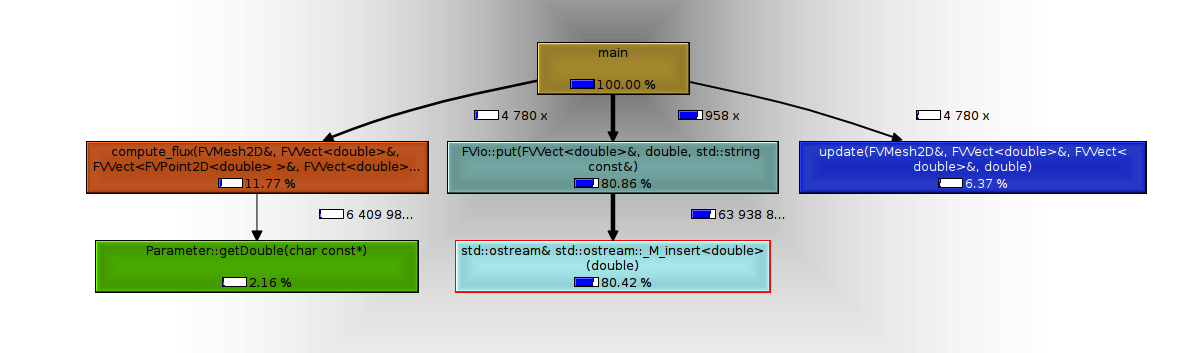
\includegraphics[width=\textwidth]{images/output.png}
\end{center}
\end{figure}

\begin{center}
\parbox{0.5\textwidth}{
\begin{itemize}
\item{81\% output}
\item{12\% \texttt{compute\_flux}}
\item{6\% \texttt{update}}
\end{itemize}
}
\end{center}
\end{frame}





\begin{frame}
	\frametitle{Call Graph (without animation)}

\begin{figure}
\begin{center}
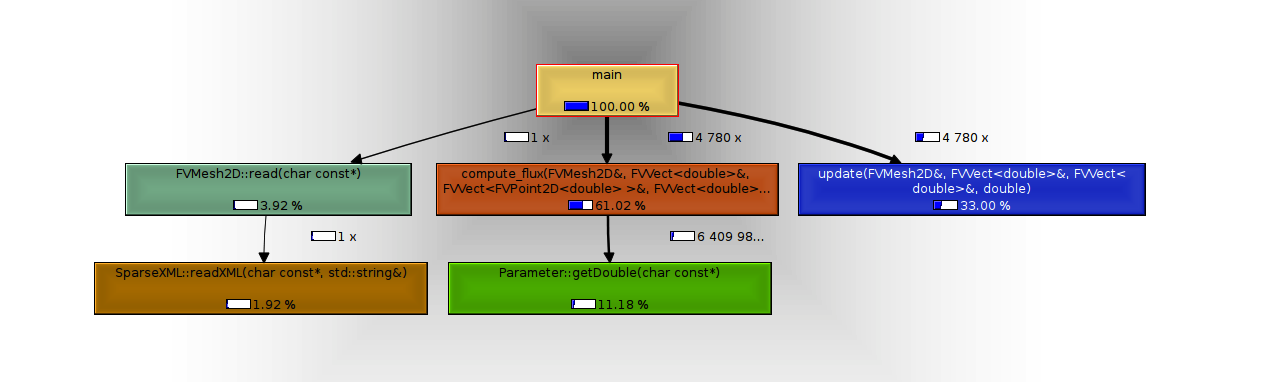
\includegraphics[width=\textwidth]{images/no_output.png}
\end{center}
\end{figure}

\begin{center}
\parbox{0.5\textwidth}{
\begin{itemize}
\item{61\% \texttt{compute\_flux}}
\item{33\% \texttt{update}}
\end{itemize}
}
\end{center}
\end{frame}











\section{Optimization \& Parallelization}
\begin{frame}
	\frametitle{Self inflicted problems}

\begin{figure}
\begin{center}
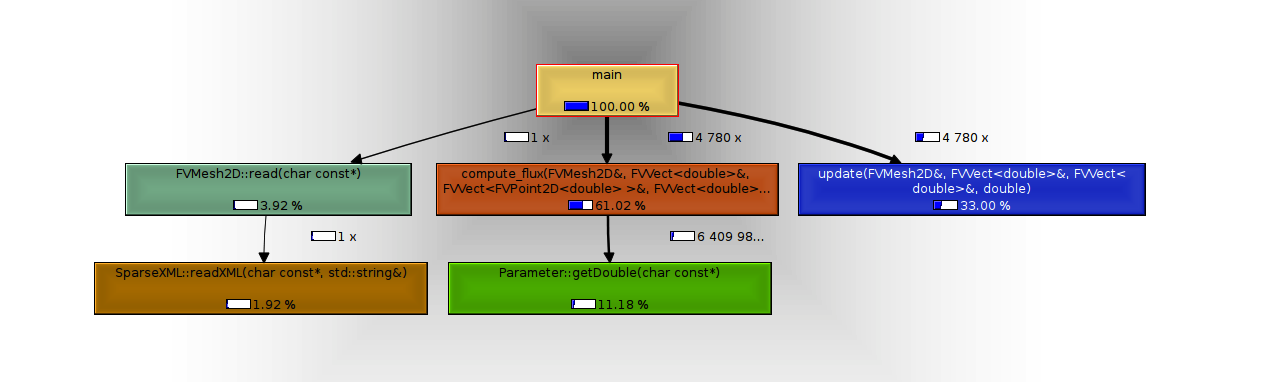
\includegraphics[width=\textwidth]{images/no_output.png}
\end{center}
\end{figure}

\begin{center}
\parbox{0.5\textwidth}{
\begin{itemize}
\item{12\% \texttt{\smaller getDouble(char const *)}}
\end{itemize}
}
\end{center}
\end{frame}







\begin{frame}
	\frametitle{It's a Pointer's World}

\lstinputlisting[language=C++]{code/pointers.cpp}

\begin{center}
\parbox{0.5\textwidth}{

\begin{itemize}
\item{Excessive dereferencing levels}
\end{itemize}
}
\end{center}

\end{frame}





\begin{frame}
	\frametitle{Dependences}

\lstinputlisting[language=C++]{code/wdependence.cpp}


\begin{center}
\parbox{0.5\textwidth}{
\begin{itemize}
\item{Dependency between iterations;}
\item{Replaced with $v_{max}$}
\item{Algorithm
		\begin{center}
		\parbox{0.5\textwidth}{\ttfamily
		While $t < t_{f}$	\\
		 |  $\Delta t \leftarrow$ compute\_flux(...)	\\
		 |  max\_reduction(...)	\\
		 |  update(...)	\\
		 |  $t \leftarrow t + \Delta t$	\\
		}
		\end{center}
		}
\end{itemize}
}
\end{center}

\end{frame}




\section{OpenMP}
\subsection{Implementation}
\begin{frame}
	\frametitle{Implementation}

\begin{itemize}
\item{Loop iteration change;}
\item{\texttt{\#pragma omp parallel for}}
\item{Reduction
	\begin{itemize}
	\item{\texttt{max} reduction in OpenMP only with GCC 4.7;}
	\item{Thread local maxima array;}
	\item{Global maximum outside the loop;}
	\end{itemize}
	}
\end{itemize}

\end{frame}





\begin{frame}
	\frametitle{Reduction \texttt{max}}

\lstinputlisting[language=C++]{code/wodependence.cpp}
\begin{center}
$\ldots$
\end{center}
\lstinputlisting[language=C++]{code/maxfor.cpp}

\end{frame}






\section{Profiling}
\subsection{Methodology}
\begin{frame}
	\frametitle{Methodology}

	SeARCH Node 201-1:
	\begin{itemize}
		\item{Intel Xeon 5130 2.0 GHz;}
		\item{Two dual-core processors;}
		\item{Cache: 32KB + 32KB (L1), 4MB (L2);}
		\item{4GB RAM;}
	\end{itemize}
	
	Test cases:
	\begin{table}
		\begin{center}
			\begin{tabular}{|l|r|c|}
			\hline
\textbf{Name	}	&	\textbf{Size}	&	\textbf{Memory Level}	\\
			\hline
			\hline
tiny		&	0.22		MB	&	L2	\\
small	&	0.92		MB	&	L2	\\
medium	&	3.82		MB	&	L2	\\
big		&	15.38	MB	&	RAM	\\
huge		&	62.36	MB	&	RAM	\\
			\hline
			\end{tabular}
		\end{center}
	\end{table}

\end{frame}






\subsection{Results --- \texttt{compute\_flux}}
\begin{frame}
	\frametitle{Time}

\begin{figure}
\begin{center}
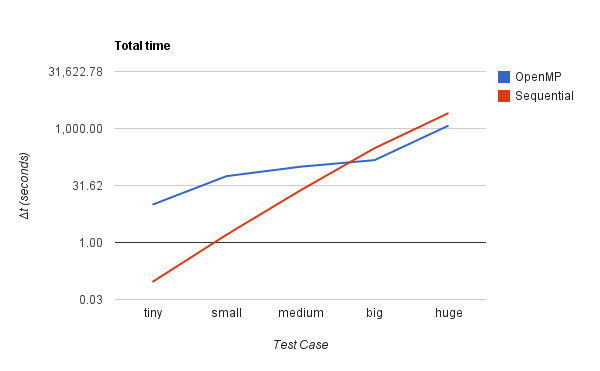
\includegraphics[width=\textwidth]{images/pfac/chrttime.png}
\end{center}
\end{figure}

\end{frame}










\begin{frame}
	\frametitle{CPI/IPC}

\begin{figure}
\begin{center}
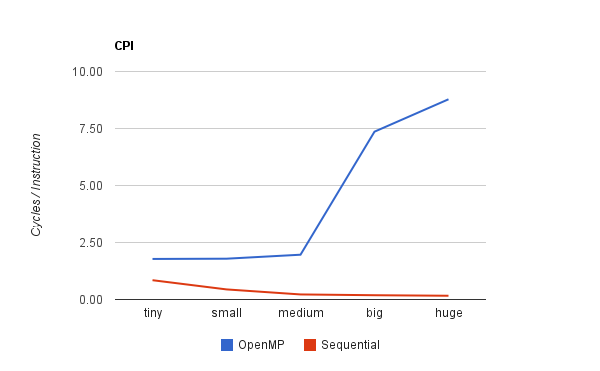
\includegraphics[width=0.5\textwidth]{images/pfac/chrtcpi.png}
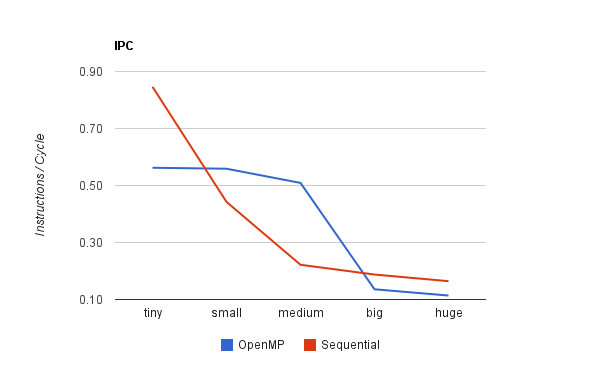
\includegraphics[width=0.5\textwidth]{images/pfac/chrtipc.png}
\end{center}
\end{figure}

\begin{itemize}
\item{Overhead effects in OpenMP;}
\item{Almost no ILP;}
\end{itemize}

\end{frame}











\begin{frame}
	\frametitle{Memory Usage}

\begin{figure}
\begin{center}
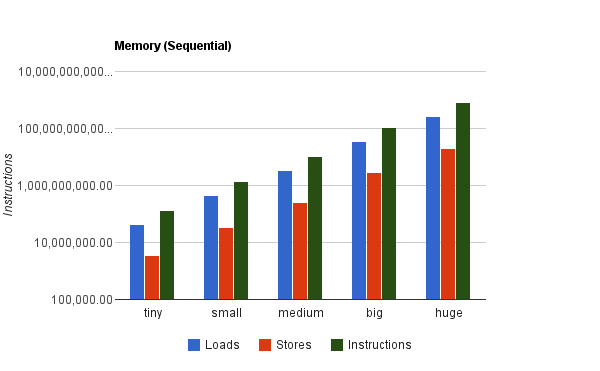
\includegraphics[width=0.5\textwidth]{images/pfac/chrtmemseq.png}
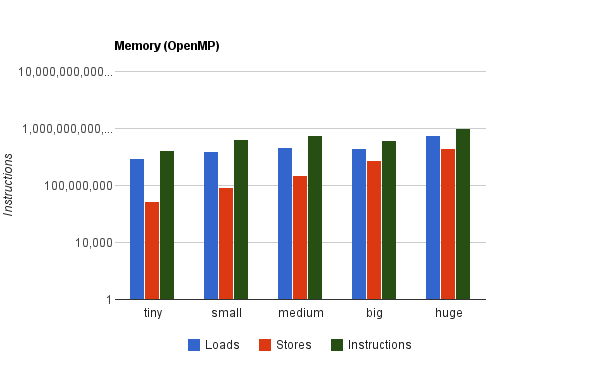
\includegraphics[width=0.5\textwidth]{images/pfac/chrtmemomp.png}
\end{center}
\end{figure}

Memory instructions ratio:
\begin{itemize}
\item{≈35\% in sequential}
\item{≈25-30\% in OpenMP}
\end{itemize}

\end{frame}









\begin{frame}
	\frametitle{Cache Miss Rates}

\begin{figure}
\begin{center}
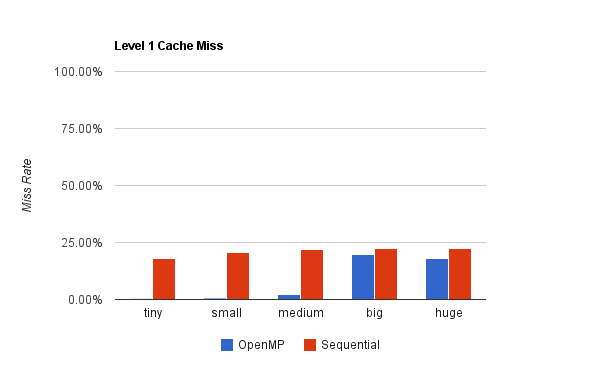
\includegraphics[width=0.5\textwidth]{images/pfac/chrtl1.png}
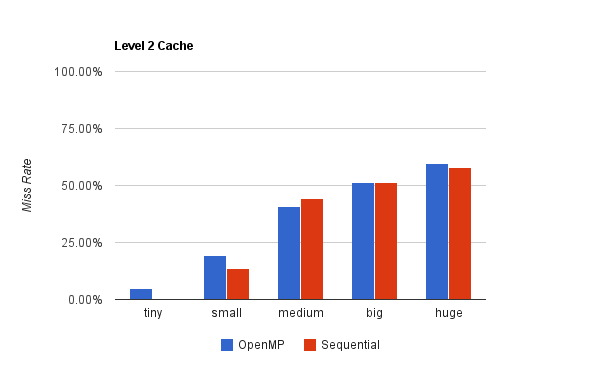
\includegraphics[width=0.5\textwidth]{images/pfac/chrtl2.png}
\end{center}
\end{figure}

\begin{itemize}
\item{L1 miss rates up to 20\%;}
\item{L2 miss rates up to 60\%;}
\end{itemize}

\end{frame}









\begin{frame}
	\frametitle{CPU Usage}

\begin{figure}
\begin{center}
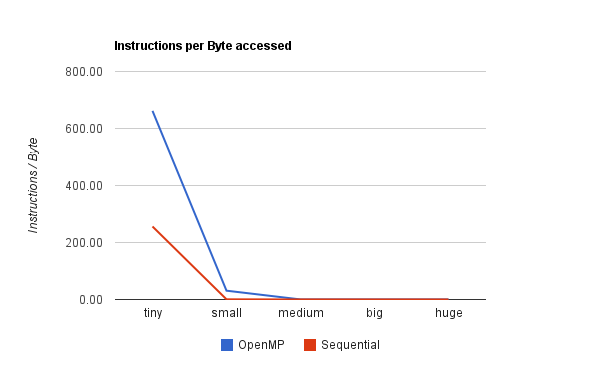
\includegraphics[width=0.5\textwidth]{images/pfac/chrtipb.png}
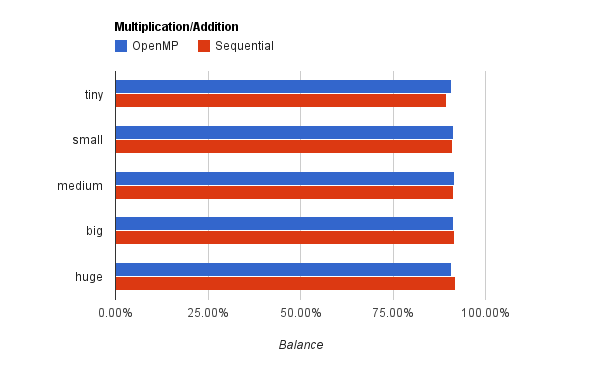
\includegraphics[width=0.5\textwidth]{images/pfac/chrtmab.png}
\end{center}
\end{figure}

\begin{itemize}
\item{Memory limitations;}
\item{≈90\% multiplication/addition balance;}
\end{itemize}

\end{frame}








\section{Conclusion}
\begin{frame}
	\frametitle{Conclusion}

\begin{itemize}
\item{Non scalable;}
\item{Bottleneck: memory;}
\item{OpenMP overhead is heavy;}
\item{PAPI overhead also very heavy;}
\item{Shared workstation generates interference;}
\item{FVLib needs a performance cleanup;}
\end{itemize}

\end{frame}



\subsection{Future Work}
\begin{frame}
	\frametitle{Future Work}

\begin{itemize}
\item{New structures:
	\begin{itemize}
	\item{Remove dereferencing;}
	\item{Improve locality;}
	\end{itemize}
	}
\item{Parallelize \texttt{update};}
\item{Time based measures:
	\begin{itemize}
	\item{Better for GPU comparison;}
	\item{Less overhead during execution;}
	\end{itemize}
	}
\end{itemize}

\end{frame}





\section{Questions}
\begin{frame}
	\titlepage
	\begin{center}
		\Huge\bfseries
		- ? -
	\end{center}
\end{frame}

\end{document}%	end presentation